\section{Estimação Paramétrica}

\subsection{Introdução}

Sabendo $P(\omega_i)$ e $p(\boldsymbol{x}|\omega_i)$ é possível projetar um classificador ótimo. Contudo, em aplicações reais de classificação de padrões raramente tem-se este conhecimento completo a respeito da estrutura probabilística do problema. Geralmente o que está disponível é um conhecimento superficial da situação e um conjunto de \textbf{dados de treinamento}.

Como exemplo, sejam 300 objetos divididos em 2 classes de modo que a classe 1 tenha 200 objetos e a classe 2 tenha 100. Cada objeto é gerado a partir de uma das 3 gaussianas bi-variadas:

\begin{description}\itemsep0pt
    \item[1a:] $\mu_1 = 60$, $\mu_2 = 30$, $\sigma_1^2 = 9$ e $\sigma_2^2 = 144$
    \item[1b:] $\mu_1 = 52$, $\mu_2 = 30$, $\sigma_1^2 = 9$ e $\sigma_2^2 = 9$
    \item[2:] $\mu_1 = 45$, $\mu_2 = 22$, $\sigma_1^2 = 100$ e $\sigma_2^2 = 9$
\end{description}

\noindent Nota-se que $\boldsymbol{\Sigma}_{1a}$, $\boldsymbol{\Sigma}_{1b}$ e $\boldsymbol{\Sigma}_2$ são matrizes diagonais, reduzindo-as a vetores de variância, o que significa independência entre as variáveis.

As duas imagems em \figureref{samples} mostram os dados de treinamento. Na de cima os dados são divididos em clusters gerados pelas gaussianas definidas anteriormente. Na segunda são dividos em duas classes.

\begin{figure}[ht]
    \centering
    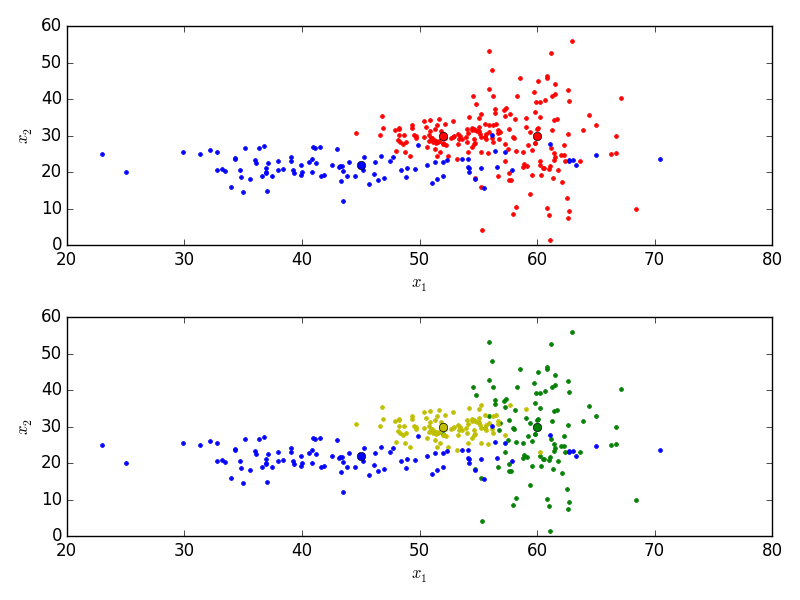
\includegraphics[width=0.5\columnwidth]{samples}
    \caption{Classes 1a (verde), 1b (amarelo) e 2 (azul).}
    \label{fig:samples}
\end{figure}

Pode-se utilizar estas amostras para estimar as probabilidades e densidades de probabilidade desconhecidas. Para problemas de aprendizagem supervisionada, a estimação das $P(\omega_i)$ é bastante simples. Sabendo a frequência relativa de aparição de cada classe $\omega_i$ no conjunto de treinamento, pode-se estimar suas $P(\omega_i)$ (desde que o conjunto de treinamento seja uma boa representação do ``mundo real"). Contudo, estimar as $p(\boldsymbol{x}|\omega_i)$ é complicado quando se tem poucos dados, especialmente quando a dimensionalidade de $\boldsymbol{x}$ aumenta. Uma maneira mais prática é assumir cada $p(\boldsymbol{x}|\omega_i)$ como uma gaussiana, cujas média e matriz de covariância são dadas por $\boldsymbol{\mu}_i$ e $\boldsymbol{\Sigma}_i$. Logo, o problema passa de estimar uma função desconhecida $p(\boldsymbol{x}|\omega_i)$ para estimar os \textbf{parâmetros} $\boldsymbol{\mu}_i$ e $\boldsymbol{\Sigma}_i$.

Para a estimação dos parâmetros, será utilizada a técnica da \textbf{máxima-verossimilhança}.

\subsection{Máxima-Verossimilhança}

Estimação por Máxima-Verossimilhança (Maximum-Likelihood, ML) considera os parâmetros como quantidades cujos valores são fixos, mas desconhecidos. A melhor estimativa de seus valores é aquela que maximiza a probabilidade de obter as amostras observadas. Este método possui uma gama de atributos atrativos. Primeiramente, possui quase sempre boas propriedades de convergência quando o número de amostras de treinamento aumenta. Além disso, ML geralmente é mais simples que métodos alternativos, tais como técnicas bayesianas.

\subsubsection*{Princípio Geral}

Um conjunto $\mathcal{D}$ de amostras é dividido em conjuntos $\mathcal{D}_1, .., \mathcal{D}_c$ cujas amostras são desenhadas independentemente, de acordo com $p(\boldsymbol{x}|\omega_j)$, resultado de variáveis aleatórias independentes e identicamente distribuídas. Assume-se que $p(\boldsymbol{x}|\omega_j)$ tem uma forma paramétrica, como por exemplo $N(\boldsymbol{\mu}_j, \boldsymbol{\Sigma}_j)$, de modo que pode ser escrita como $p(\boldsymbol{x}|\omega_j, \boldsymbol{\theta}_j)$, onde $\boldsymbol{\theta}_j$ consiste nos componentes de $\boldsymbol{\mu}_j$ e $\boldsymbol{\Sigma}_j$. O problema torna-se utilizar as informações dadas pelas amostras para obter boas estimativas dos vetores desconhecidos $\boldsymbol{\theta}_j$, para cada $\omega_j$. Uma simplificação é assumir que as amostras de cada $\mathcal{D}_j$ provêem informações relevantes apenas aos seus respectivos $\boldsymbol{\theta}_j$.

\begin{figure}[ht]
    \centering
    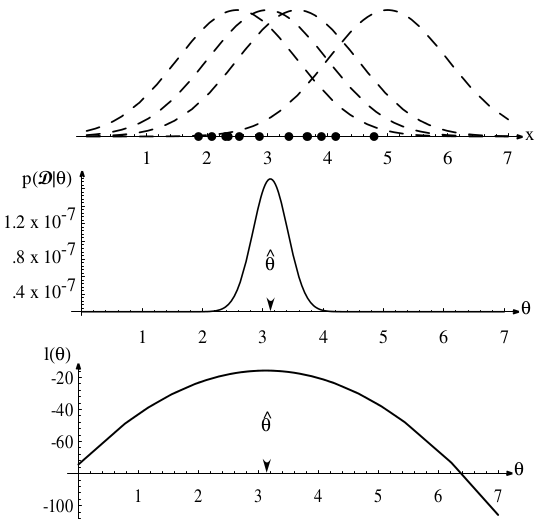
\includegraphics[width=0.5\columnwidth]{maximum-likelihood}
    \caption{Estimação do parâmetro $\boldsymbol{\hat{\theta}}$, o valor $\boldsymbol{\hat{\theta}}$ achado e $l(\boldsymbol{\hat{\theta}})$.}
    \label{fig:maximum-likelihood}
\end{figure}

Usa-se o conjunto $\mathcal{D}$, composto pelas amostras de treinamento $\boldsymbol{x}_1, ..., \boldsymbol{x}_n$ desenhadas independentemente de $p(\boldsymbol{x}|\boldsymbol{\theta})$, para estimar os $\boldsymbol{\theta}$ desconhecidos, tal que

\begin{equation}
    p(\mathcal{D}|\boldsymbol{\theta}) = \prod_{k=1}^{n} p(\boldsymbol{x}_k|\boldsymbol{\theta}).
    \label{eq:pdf_D}
\end{equation}

\noindent A densidade $p(\mathcal{D}|\boldsymbol{\theta})$ é conhecida como a \textbf{verossimilhança} de $\boldsymbol{\theta}$ em relação às amostras, e sua estimativa máxima é, por definição, o valor $\boldsymbol{\hat{\theta}}$ que maximiza  $p(\mathcal{D}|\boldsymbol{\theta})$ (\figureref{maximum-likelihood}).

Devido a ser monotonicamente crescente e mais fácil de trabalhar que a verossimilhança, o uso da log-verossimilhança

\begin{equation}
    l(\boldsymbol{\theta}) \equiv \ln p(\mathcal{D}|\boldsymbol{\theta}) = \sum_{k=1}^{n} \ln p(\boldsymbol{x}_k|\boldsymbol{\theta})
    \label{eq:log_likelihood}
\end{equation}

\noindent é preferível. Logo, a solução para $\boldsymbol{\hat{\theta}}$ é

\begin{equation}
    \boldsymbol{\hat{\theta}} = \arg\max_{\boldsymbol{\theta}} l(\boldsymbol{\theta}),
    \label{eq:hat_theta}
\end{equation}

\noindent onde a dependencia do conjunto de dados $\mathcal{D}$ fica implícito. Se o número de parametros a serem estimados é $p$, então $\boldsymbol{\theta} = (\theta_1, ..., \theta_p)^t$ e $\boldsymbol{\nabla}_{\boldsymbol{\theta}} = (\frac{\partial}{\partial \theta_1}, ..., \frac{\partial}{\partial \theta_p})^t$, e, pela \equationref{log_likelihood}

\begin{equation}
    \boldsymbol{\nabla}_{\boldsymbol{\theta}} l = \sum_{k=1}^{n} \boldsymbol{\nabla}_{\boldsymbol{\theta}} \ln p(\boldsymbol{x}_k|\boldsymbol{\theta}).
    \label{eq:gradient_theta_log}
\end{equation}

Então, um conjunto de condições necessárias para a estimação da máxima verossimilhança para $\boldsymbol{\theta}$ pode ser obtido do conjunto de $p$ equações

\begin{equation}
    \boldsymbol{\nabla}_{\boldsymbol{\theta}} l = \boldsymbol{0}.
    \label{eq:gradient_theta_log_equal_zero}
\end{equation}

Uma solução $\boldsymbol{\hat{\theta}}$ para \equationref{gradient_theta_log_equal_zero} pode ser uma máximo global, um máximo/mínimo local, ou (raramente) um ponto de inflexão de $l(\boldsymbol{\theta})$. Se todas as soluções forem achadas, é garantido que representa o máximo verdadeiro, senão deve-se checar todas as soluções individualmente (ou calcular derivadas de segunda ordem) para identificar qual é o ótimo global.

\subsubsection*{Gaussiana com $\boldsymbol{\mu}$ desconhecido}

Neste caso o vetor $\boldsymbol{\theta} = \boldsymbol{\mu}$, levando a $l(\boldsymbol{\theta}) = l(\boldsymbol{\mu}) \equiv \ln p(\mathcal{D}|\boldsymbol{\mu})$. Logo pela \equationref{log_likelihood},

\begin{equation}
    l(\boldsymbol{\mu}) = \sum_{k=1}^{n} \ln p(\boldsymbol{x}_k|\boldsymbol{\mu}),
    \label{eq:log_mu}
\end{equation}

\noindent e pela \equationref{gradient_theta_log},

\begin{equation}
    \boldsymbol{\nabla}_{\boldsymbol{\mu}} l = \sum_{k=1}^{n} \boldsymbol{\nabla}_{\boldsymbol{\mu}} \ln p(\boldsymbol{x}_k|\boldsymbol{\mu}).
    \label{eq:nabla_mu_log}
\end{equation}

\noindent Como $\boldsymbol{\nabla}_{\boldsymbol{\mu}} \ln p(\boldsymbol{x}_k|\boldsymbol{\mu}) = \boldsymbol{\Sigma}^{-1} (\boldsymbol{x}_k - \boldsymbol{\mu})$ e $\boldsymbol{\nabla}_{\boldsymbol{\mu}} l = 0$ (\equationref{gradient_theta_log_equal_zero}), então

\begin{equation}
    \sum_{k=1}^{n} \boldsymbol{\Sigma}^{-1} (\boldsymbol{x}_k - \boldsymbol{\hat{\mu}}) = \boldsymbol{0}.
    \label{eq:nabla_mu_log_equals_zero}
\end{equation}

\noindent Multiplicando por $\boldsymbol{\Sigma}$ e rearranjando os termos, tem-se

\begin{equation}
    \boldsymbol{\hat{\mu}} = \frac{1}{n} \sum_{k=1}^{n} \boldsymbol{x}_k.
    \label{eq:mu_optimum_case_1}
\end{equation}

Fica evidente que para o caso em que apenas $\boldsymbol{\mu}$ é desconhecido, a estimativa para a máxima verossimilhança é apenas a média das amostras, às vezes escrita como $\boldsymbol{\hat{\mu}}_n$ para clarificar sua dependência do número de amostras.

\subsubsection*{Gaussiana com $\boldsymbol{\mu}$ e $\boldsymbol{\Sigma}$ desconhecidos}

Este é o caso mais típico, quando $\boldsymbol{\mu}$ e $\boldsymbol{\Sigma}$ são desconhecidos. Desta forma, este parâmetros constituem as componentes do vetor paramétrico $\boldsymbol{\theta}$, ou seja $\boldsymbol{\theta} = (\boldsymbol{\mu}, \boldsymbol{\Sigma})^t$. Considerando o caso univariado, $\theta_1 = \mu$ e $\theta_2 = \sigma^2$. Então

\begin{equation}
    \ln p(x_k|\boldsymbol{\theta}) = -\frac{1}{2} \ln 2\pi\theta_2 - \frac{1}{2\theta_2}(x_k - \theta_1)^2
    \label{eq:log_likelihood_mu_sigma_univar}
\end{equation}

\noindent e seu gradiente é

\begin{equation}
    \boldsymbol{\nabla}_{\boldsymbol{\theta}} l = \boldsymbol{\nabla}_{\boldsymbol{\theta}} \ln p(x_k|\boldsymbol{\theta}) = \tworowsmatrix{\frac{1}{\theta_2}(x_k - \theta_1)}{-\frac{1}{2\theta_2} + \frac{(x_k - \theta_1)^2}{2\theta_2^2}}
    \label{eq:grad_log_likelihood_mu_sigma_univar}
\end{equation}

\noindent e pela \equationref{nabla_mu_log_equals_zero} tem-se

\begin{equation}
    \sum_{k=1}^n \frac{1}{\hat{\theta_2}}(x_k - \hat{\theta_1}) = 0
    \label{eq:grad_log_likelihood_mu_sigma_univar_theta_1}
\end{equation}

\noindent e

\begin{equation}
    -\sum_{k=1}^n \frac{1}{2\hat{\theta_2}} + \sum_{k=1}^n \frac{(x_k - \hat{\theta_1})^2}{2\hat{\theta_2}^2} = 0,
    \label{eq:grad_log_likelihood_mu_sigma_univar_theta_2}
\end{equation}

\noindent Rearrumando tudo, tem-se

\begin{equation}
    \hat{\mu} = \frac{1}{n} \sum_{k=1}^n x_k
    \label{eq:mu_optimum_case_2}
\end{equation}

\noindent e

\begin{equation}
    \hat{\sigma}^2 = \frac{1}{n} \sum_{k=1}^n (x_k - \hat{\mu})^2.
    \label{eq:sigma_optimum_case_2}
\end{equation}

Dando um salto de fé (embora esta seja demonstrável, diferente da cristã) e trocando os $\hat{\mu}$ e $\hat{\sigma}$ por $\boldsymbol{\hat{\mu}}$ e $\boldsymbol{\hat{\Sigma}}$, respectivamente, tem-se

\begin{equation}
    \boldsymbol{\hat{\mu}} = \frac{1}{n} \sum_{k=1}^n \boldsymbol{x}_k
    \label{eq:bold_mu_optimum_case_2}
\end{equation}

\noindent e

\begin{equation}
    \boldsymbol{\hat{\Sigma}} = \frac{1}{n} \sum_{k=1}^n (\boldsymbol{x}_k - \boldsymbol{\hat{\mu}})(\boldsymbol{x}_k - \boldsymbol{\hat{\mu}})^t.
    \label{eq:bold_sigma_optimum_case_2}
\end{equation}